\chapter{TEOR\'{I}A: Plegamiento y din\'{a}mica de macromol\'{e}culas} \label{macro2}

Ahora que conocemos de qu\'{e} est\'{a}n hechas las macromol\'{e}culas y sabemos lo importantes que son 
en biolog\'\i{}a, haremos un peque\~no repaso sobre las ideas centrales del proceso de plegamiento
(\italics{folding}), responsable de que estas mol\'{e}culas adquieran la estructura tridimensional 
que les confiere su funci\'{o}n.

\section{Plegamiento y desnaturalizaci\'{o}n} \label{desnat}

El inter\'{e}s sobre el plegamiento de las macromol\'{e}culas se despert\'{o} al estudiar sus reacciones
de desnaturalizaci\'{o}n. Si tenemos prote\'\i{}nas o \'{a}cidos nucleicos en disoluci\'{o}n y cambiamos de 
forma notable las condiciones en que suelen encontrarse en su medio biol\'{o}gico, pierden su 
estructura y funci\'{o}n nativas. Este proceso, llamado reacci\'{o}n de desnaturalizaci\'{o}n, puede ser 
reversible en ciertas condiciones y los cambios pueden ser por ejemplo de temperatura, por 
encima de su temperatura de fusi\'{o}n ($T_{m}$), o en la naturaleza del solvente.\\ 

\citet{Anfinsen1961} mostr\'{o} experimentalmente que la desnaturalizaci\'{o}n es reversible al menos para 
prote\'\i{}nas peque\~nas, a\~nadiendo y retirando agentes desnaturalizantes a disoluciones de enzimas 
que ganaban y perd\'\i{}an su actividad. As\'\i{} demostr\'{o} que el plegamiento de una prote\'\i{}na depende 
exclusivamente de su secuencia, aunque hoy sabemos que algunas necesitan la ayuda de 
chaperoninas \citep{Hartl2002}.\\

Todav\'{i}a hoy el proceso de plegamiento no se comprende bien debido a su complejidad 
(ver secciones \ref{complejidad} y \ref{complejidad2}), aunque llevemos 50 a\~{n}os estudi\'{a}ndolo \citep{Dill2012}.
%Para hacerse una idea de su complejidad y de todo el trabajo realizado en este campo una buena introducci\'{o}n puede ser el trabajo
%\htmladdnormallink{trabajo}{./papers/Rosefolding2006.pdf} 
%de \cite{Rose2006}.

\begin{figure}
%\htmlimage{scale=1.0}
\begin{center} 
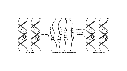
\includegraphics{desnatADN}
\caption%[]
{
Reacci\'{o}n de desnaturalizaci\'{o}n y renaturalizaci\'{o}n (hibridaci\'{o}n) de una mol\'{e}cula de ADN,
tomada de \citet{HernandezLemus2012} y reproducido con permiso de los autores.
}
\label{fig:desnatADN}
\end{center}
\end{figure}

La $T_{m}$ de los \'{a}cidos nucleicos es proporcional al contenido en bases GC de su secuencia, 
ya que estos pares de bases (ver figura \ref{fig:est2adn}) establecen entre s\'\i{} 3 puentes de hidr\'{o}geno, 
mientras que los AT/AU s\'{o}lo 2. Si la temperatura supera $T_{m}$, las mol\'{e}culas de ADN se separan 
en dos hebras polinucleot\'\i{}dicas (como se muestra en la figura \ref{fig:desnatADN}), pero si la 
bajamos lentamente ambas hebras vuelven a unirse de forma complementaria en una reacci\'{o}n llamada 
hibridaci\'{o}n. De nuevo vemos c\'{o}mo en este caso la secuencia es suficiente para guiar el plegamiento, 
al menos para mol\'{e}culas peque\~nas.\\

\section{Fuerzas que influyen en el proceso de plegamiento de macromol\'{e}culas}

Se han reconocido varias propiedades e interacciones f\'\i{}sicas que gu\'\i{}an al proceso de plegamiento, 
como las que mencionamos en la secci\'{o}n \ref{macro1:intnocov}. Algunas son espec\'\i{}ficas
del plegamiento de prote\'\i{}nas, como la formaci\'{o}n de enlaces disulfuro entre ciste\'\i{}nas o la formaci\'{o}n
de puentes salinos entre amino\'{a}cidos b\'{a}sicos y \'{a}cidos, pero en general se acepta que las principales
son la hidrofobicidad en un medio acuoso y la formaci\'{o}n de puentes de hidr\'{o}geno 
\citep{Dill1990,Lehninger1982,Mathews1999}.

Algunas de estas propiedades pueden estimarse directamente desde la secuencia. Por ejemplo, se han
propuesto escalas de hidrofobicidad como la de la tabla siguiente, %\ref{tab:hidrof}, 
que quedan englobadas en clasificaciones de amino\'{a}cidos como la de secci\'{o}n \ref{fig:amino_classif}.

\begin{table}[h]
\begin{center}
\begin{scriptsize}
\begin{tabular}{|l|l|l|l|}\hline
A & 1.8 & M & 1.9\\   
C & 2.5 & N & -3.5\\
D & -3.5 & P & -1.6\\ 
E & -3.5 & Q & -3.5\\  
F & 2.8 & R & -4.5\\
G & -0.4 & S & -0.8\\      
H & -3.2 & T & -0.7\\    
I & 4.5 & V & 4.2\\   
K & -3.9 & W & -0.9\\
L & 3.8 & Y & -1.3\\
\end{tabular}
\end{scriptsize}
\end{center}
\caption%[]
{Escala de hidrofobicidad de los 20 amino\'{a}cidos, con valores positivos para los residuos hidrof\'{o}bicos
y negativos para los dem\'{a}s \citep{Kyte1982}.}
\label{tab:hidrof}
\end{table} 

Como resultado del proceso de plegamiento en medios acuosos, las macromol\'{e}culas se empaquetan mostrando 
hacia el solvente superficies hidrof\'\i{}licas y ocultando los componentes m\'{a}s hidrof\'{o}bicas. En el interior
las interacciones de van der Waals dan estabilidad al conjunto. Como siempre, hay excepciones notables \citep{Sun2014}.
En el caso de las prote\'\i{}nas otro factor que condiciona el plegamiento es su tendencia natural a formar 
mult\'\i{}meros \citep{Garcia2017}. 
%Recientemente se ha calculado 
%\citep{Voss2005} que el empaquetamiento en el interior de mol\'{e}culas de RNA es m\'{a}s compacto que el de 
%las prote\'\i{}nas. 

\section{Complejidad algor\'\i{}tmica del plegamiento} \label{complejidad}

Sabemos que bajo condiciones fisiol\'{o}gicas el proceso de plegamiento es termodin\'{a}micamente
favorable, es decir, que las macromol\'{e}culas son m\'{a}s estables en su conformaci\'{o}n nativa que en
otras posibles conformaciones. Y conocemos al menos los factores m\'{a}s importantes que afectan
y gu\'\i{}an al proceso de plegamiento. Por \'{u}ltimo, sabemos que el plegamiento es un proceso r\'{a}pido,
que tarda a lo sumo tiempos del orden de segundos. A pesar de esto, a d\'\i{}a de hoy no sabemos 
predecir de forma precisa c\'{o}mo se plegar\'{a} una prote\'\i{}na o un \'{a}cido nucleico partiendo solamente 
de su secuencia. 

Cu\'{a}les son las dificultades? Esto lo veremos tomando como ejemplo las prote\'\i{}nas, que se han estudiado
mucho m\'{a}s a este nivel. Son fundamentalmente dos:
\begin{itemize}
\item el enorme n\'{u}mero de posibles conformaciones que puede tomar una cadena polipept\'\i{}dica
\item la necesidad de cuantificar la estabilidad en  condiciones fisiol\'{o}gicas de cada una de ellas
\end{itemize}

El proceso de plegamiento puede entonces verse como una exploraci\'{o}n en un embudo (\italics{funnel}) como el de la figura
\ref{fig:foldfunnel}, donde observamos un m\'{a}ximo de estabilidad que se corresponde con un m\'{i}nimo de energ\'{i}a libre
(conformaciones nativas), y otros m\'{a}ximos secundarios o locales denominados estados metaestables. En ciertas condiciones
las prote\'{i}nas pueden quedarse atrapadas en estos estados y perder funcionalidad o agregarse, 
de ah\'{i} la importancia de las chaperonas \citep{pascual_garcia_alberto_2014_1066348}.
%que hay que descartar en la b\'{u}squeda,puesto que no se corresponden con la estructura nativa.

\begin{figure}
\begin{center} 
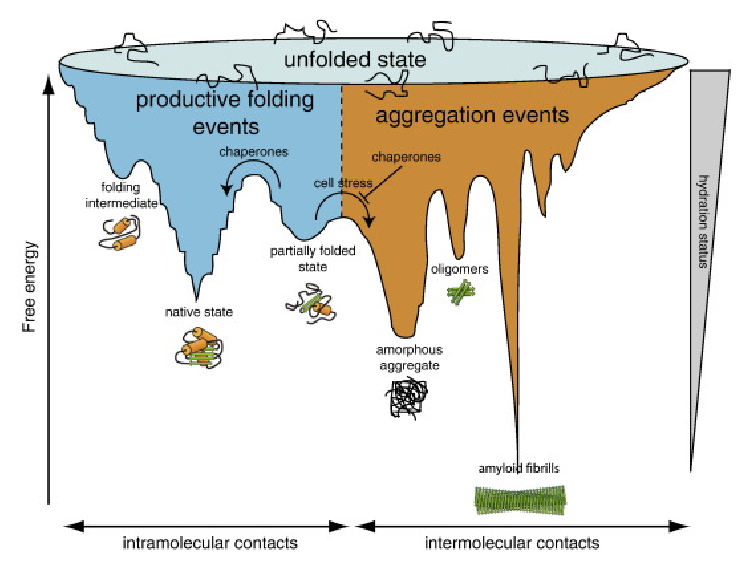
\includegraphics[]{funnel2}
\caption%[]
{
Superficie energ\'{e}tica del plegamiento de prote\'\i{}nas desde su s\'\i{}ntesis hasta su estado final plegado o agregado. 
Algunas conformaciones metaestables deben superar barreras energ\'{e}ticas para retomar su ruta de plegamiento favorable,
en ocasiones con ayuda de chaperonas (izquierda). Cuando varias mol\'{e}culas se pliegan en el mismo compartimento pueden formar contactos
que propicien la acumulaci\'{o}n de agregados amorfos, olig\'{o}meros t\'{o}xicos o fibrillas amiloides (derecha).
Figura tomada de \citet{Amm2014} y reproducida con permiso de los autores.
}
\label{fig:foldfunnel}
\end{center}
\end{figure}

\begin{figure}
\begin{center} 
\includegraphics[width=0.4\textwidth]{per_residue_folding}
\caption%[]
{
Contribuciones de cada uno de los residuos de una prote\'\i{}na camale\'{o}nica, que puede adoptar 
un plegamiento $\alpha$ (izquierda) u otro $\alpha + \beta$ (derecha) con muy pocos cambios en la secuencia.
Arriba: los residuos que favorecen el plegamiento se empaqueten en la estructura globular correspondiente. 
Medio: las medidas de energ\'\i{}a libre por residuo revelan las partes de la secuencia que favorecen el plegamiento. 
Abajo: la energ\'\i{}a libre por residuo puede generalmente atribuirse a la secuencia (GA30 o GB30) que favorece cada plegamiento. 
Figura tomada de \citet{Roy2014} y reproducida con permiso de los autores.
}
\label{fig:per_residue_folding}
\end{center}
\end{figure}

\begin{figure}
\begin{center} 
\includegraphics{ribozymeFolding}
\caption%[]
{
Embudo de plegamiento de una ribozima.
Figura de \citet{Behrouzi2012} y reproducida con permiso de los autores.
}
\label{fig:foldfunnelRNA}
\end{center}
\end{figure}

Desde este punto de vista, la b\'{u}squeda de la conformaci\'{o}n nativa es como buscar una aguja en un pajar. 
C\'{o}mo es el espacio de conformaciones? Lo veremos por medio de la paradoja de Levinthal.

\section{Paradoja de Levinthal} \label{complejidad2}

En una prote\'\i{}na los enlaces pept\'\i{}dicos son r\'\i{}gidos pero hay 2 enlaces libres de girar por cada amino\'{a}cido,
a parte de que cada cadena lateral puede orientarse de diferentes maneras. Parece por tanto que realmente 
es una cadena muy flexible, que puede adoptar muchas conformaciones diferentes.
\htmladdnormallink{Cyrus Levinthal}{http://en.wikipedia.org/wiki/Levinthal's_Paradox}, en 1969, fue el primero 
en hacer una estimaci\'{o}n. El razonamiento es la siguiente: 
\begin{itemize}
\item  digamos que cada amino\'{a}cido de una cadena puede tomar $X$ estados diferentes
\item una prote\'\i{}na de tama\~no medio tiene, digamos, 100 amino\'{a}cidos
\item digamos que cada cambio de estado en un medio fisiol\'{o}gico tarda un tiempo $t$
\item entonces el tiempo $T_{expl}$ que llevar\'\i{}a explorar todos los estados ser\'\i{}a de $t X^{100}$
\end{itemize}

Para $X$ peque\~nos, como $10$, y tiempos muy cortos, como $10^{-13} s$, 
$T_{expl} = 10^{-13} 10^{100} = 10^{87}s$. Ahora comp\'{a}rese este valor con los $5s$ que tarda la 
bacteria \italics{Escherichia coli} en sintetizar una prote\'\i{}na de 100 residuos completamente funcional.

Levinthal concluy\'{o} que las prote\'\i{}nas naturales no se pliegan siempre, % en su conformaci\'{o}n m\'{a}s estable, 
pues no tienen tiempo de explorar extensivamente todas las conformaciones. 
Propuso que hay otras conformaciones cercanas igualmente funcionales en t\'{e}rminos
fisiol\'{o}gicos. En la actualidad esto se ha interpretado adem\'{a}s como una evidencia de que el plegamiento no
es totalmente aleatorio, sino que es un proceso por etapas, que reduce en muchos \'{o}rdenes de magnitud 
la b\'{u}squeda de conformaciones \citep{Mathews1999,Burra2009,Sali1994}.

\section{Aproximaciones a la velocidad de plegamiento de prote\'\i{}nas} \label{hora2:K}

Desde un punto de vista qu\'{i}mico podr\'{i}amos definir el proceso de plegamiento (P) como una reacci\'{o}n, opuesta a la 
desnaturalizaci\'{o}n (D), en estos t\'{e}rminos (donde $k$ es la constante de equilibrio):
\begin{equation}
k_{d}/k_{p}=[prot_{D}]/[prot_{P}] = k
\end{equation}

Independientemente de que no sepamos todav\'\i{}a plegar 
prote\'\i{}nas con precisi\'{o}n, s\'\i{} que podemos 
en ciertos casos estimar cuanto tardar\'{a}n en plegarse a partir de su secuencia. \citet{Plaxco1998}
demostraron que la velocidad de plegamiento ($k_{p}$) de dominios est\'{a} estrechamente correlacionada con
el \italics{orden de contactos} (CO), es decir, la media de separaci\'{o}n en secuencia entre residuos del dominio
ya plegado que est\'{a}n en estrecho contacto. En la siguiente ecuaci\'{o}n N son los contactos totales, 
$S_{ij}$ es la separaci\'{o}n en secuencia entre los residuos $i,j$ y $L$ es lo longitud de la secuencia.
Se da un contacto cuando dos \'{a}tomos pesados (no H) de dos residuos se encuentran a menos de 6\AA:

\begin{equation}
CO = LN \sum_{i=1}^{L} \sum_{j=1}^{L} N S_{ij}
\end{equation}

Por otro lado, \citet{SSfoldingrate2003} encontraron otra fuerte correlaci\'{o}n entre el contenido
en estructura secundaria de una secuencia de amino\'{a}cidos, su longitud, y su velocidad de plegamiento.
La funci\'{o}n que definen tiene esta forma (donde H, T y B son fracciones de residuos en esos estados de
estructura secundaria y $L$ es la longitud de la secuencia):
%estructura secundaria (ver tabla \ref{tab:SS8}) y $L$ es la longitud de la secuencia):

\begin{equation}
ln(k_{p}) = 8{.}9T + 14H + 5{.}5B + \frac{121{.}4}{L} - 2{.}8
\end{equation}

donde $k_{p}$ se mide en $1/s^{6}$. Estas correlaciones sugieren que el factor limitante del proceso 
de plegamiento es la formaci\'{o}n de elementos de estructura secundaria.

El problema de estos m\'{e}todos es que exigen conocer la estructura de la prote\'\i{}na en cuesti\'{o}n, aunque
se podr\'\i{}an aplicar usando predicciones de estructura secundaria y de orden de contactos. 

\begin{figure}
\begin{center} 
\includegraphics[width=0.5\textwidth]{goldentriangle}
\caption%[]
{
La velocidad de plegamiento medida experimentalmente para muchas prote\'\i{}nas se ci\~{n}e a una regi\'{o}n triangular.
$L$ es la longitud en residuos de cada secuencia estudiada. Figura de \citet{Garbuzynskiy2013}, reproducida con permiso de los autores.
}
\label{fig:goldentriangle}
\end{center}
\end{figure}


\section{Algoritmos de din\'{a}mica molecular y plegamiento} \label{macro3}
 
Llegados a este punto ya podemos estudiar los principales algoritmos que se han aplicado al problema
del plegamiento y la predicci\'{o}n de estructura de macromol\'{e}culas. Podemos clasificarlos por el nivel 
de detalle que utilizan. La escala va desde m\'{e}todos que modelan cada uno de los \'{a}tomos de 
las macromol\'{e}culas en cuesti\'{o}n y del solvente en que se encuentran, hasta m\'{e}todos donde se manejan amino\'{a}cidos
o incluso elementos de estructura secundaria como un todo indivisible y se ignora o modela de forma impl\'\i{}cita el 
solvente. Se pueden ampliar estos contenidos en \citep{pascual_garcia_alberto_2014_1066348}.

\subsection{Modelos bidimensionales de plegamiento de prote\'\i{}nas}
Los primeros modelos bidimensionales \citep{Dill1995,MorenoHernandez2012,Shakhnovich1993}, que usan un alfabeto reducido donde los
amino\'{a}cidos son polares (P) o hidrof\'{o}bicos (H) y donde las cadenas se pliegan en una malla bidimensional, sirvieron
para aproximarse al plegamiento de una forma simplificada. En general se acepta que estos 
modelos reproducen las caracter\'\i{}sticas m\'{a}s importantes del proceso de plegamiento real con la ventaja 
de ser m\'{a}s manejables:
\begin{itemize}
\item se forman estructuras secundarias, que limitan la velocidad del proceso
\item el plegamiento se hace por etapas y est\'{a} dominado por la hidrofobicidad
\end{itemize}

Vamos a definir m\'{a}s formalmente este modelo, porque ilustra de forma sencilla los algoritmos de din\'{a}mica molecular
que mencionaremos en la siguiente secci\'{o}n:

\begin{itemize}
\item dado el alfabeto \{H,P\}, una prote\'\i{}na es una secuencia de longitud N, 
tal como \texttt{HHHPPPHHPPPPPHHHPPPPHHH}.
\item las prote\'\i{}nas viven en una malla bidimensional, como la de la figura \ref{fig:dillmodel}, donde cada posici\'{o}n no
puede estar ocupada por m\'{a}s de un residuo.
\item cada celda de la malla tiene 4 vecinos: N, S, E y O.
\item cada residuo est\'{a} dado en coordenadas internas empezando por el extremo, por ejemplo el residuo 2 est\'{a} al N del 1.
\item hay por lo tanto un m\'{a}ximo de $4^{N}$ conformaciones posibles.
\item no se admiten cruces en la secuencia.
\item cuando dos residuos no contiguos en secuencia ocupan celdas vecinas se dice que interaccionan.
\item la energ\'\i{}a de cada interacci\'{o}n se eval\'{u}a usando la matriz de la tabla siguiente. %\ref{tab:matrizHP}.
\item la conformaci\'{o}n nativa es aquella que minimiza la energ\'\i{}a total, maximizando la estabilidad. %en soluci\'{o}n.
\end{itemize}

\begin{figure}
\htmlimage{scale=1.0}
\begin{center} 
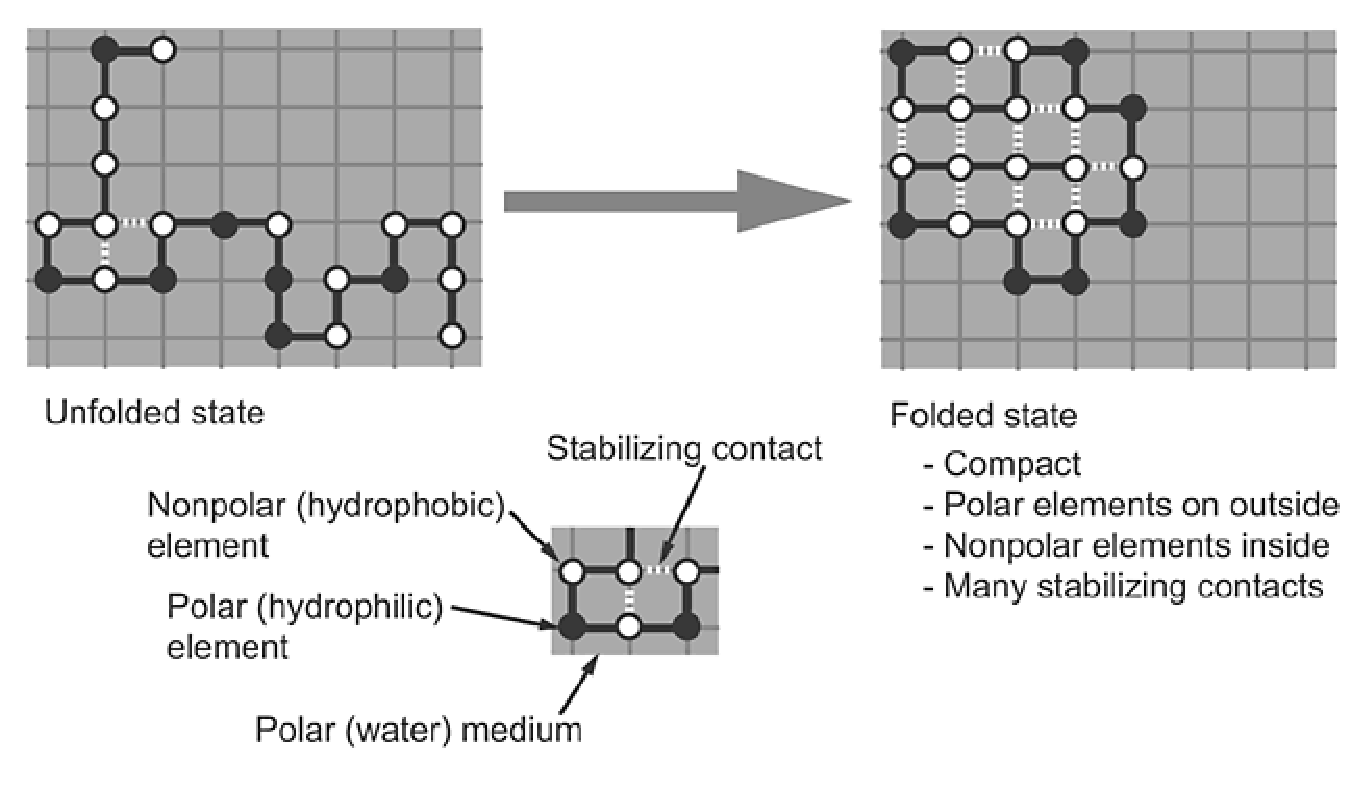
\includegraphics{dillmodel}
\caption%[]
{
Plegamiento en dos dimensiones en el modelo HP de \citet{Dill1995}. Copyright (1995) Protein Science.
}
\label{fig:dillmodel}
\end{center}
\end{figure}

\begin{table}[h]
\begin{center}
\begin{tabular}{|l|l|l|}\hline
 & P & H\\   
P & 0 & -1\\
H & -1 & -3\\ 
\end{tabular}
\end{center}
\caption%[]
{Matriz de interacci\'{o}n $M_{ij}$ en un modelo HP, que favorece expl\'{i}citamente las interacciones polares.}
\label{tab:matrizHP}
\end{table} 

\begin{figure}
\begin{center} 
\includegraphics{snake}
\caption%[]
{
Ampliaci\'{o}n del modelo de Dill a tres dimensiones implementada en el juego SNAKE de \citet{Nido2016}.
Debajo se muestran matrices de contactos correspondientes a algunos de los plegamientos. 
Figura reproducida con permiso de los autores.
}
\label{fig:snakefold}
\end{center}
\end{figure}


\subsection{Modelos tridimensionales de mec\'{a}nica molecular} \label{DM}

Los modelos tridimensionales de la \htmladdnormallink{mec\'{a}nica molecular}{http://es.wikipedia.org/wiki/Modelado_molecular}
son conceptualmente similares al modelo HP, pero en espacios tridimensionales, normalmente considerando al solvente de forma 
expl\'\i{}cita o impl\'\i{}cita y los enlaces entre \'{a}tomos (o grupos de \'{a}tomos) como muelles gobernados por la ley de 
\htmladdnormallink{Hooke}{http://es.wikipedia.org/wiki/Ley_de_elasticidad_de_Hooke}. En estos modelos, la energ\'{i}a asociada 
a la conformaci\'{o}n
de una mol\'{e}cula se calcula en un \htmladdnormallink{campo de fuerzas}{http://en.wikipedia.org/wiki/Force_field_(chemistry)}.
De esta manera, para cada conformaci\'{o}n molecular se puede calcular su energ\'{i}a potencial por medio de funciones que 
incluyen t\'{e}rminos que consideran las longitudes y \'{a}ngulos de los enlaces, 
las torsiones entre grupos vecinos (diedros) y las interacciones no covalentes entre \'{a}tomos (Van der Waals, Coulomb y puentes de H por ejemplo):

\begin{equation}
potencial(r_{N}) = w_{1} \cdot enlaces(r_{N}) + w_{2} \cdot \acute{a}ngulos(r_{N}) + w_{3} \cdot torsiones(r_{N}) + w_{4} \cdot interacciones(r_{N})
\label{eq:PnR}
\end{equation} 

donde $w_{1},w_{2},w_{3},w_{4}$ son los pesos de cada t\'{e}rmino y 
$r_{N}$ las coordenadas de $N$ \'{a}tomos de la mol\'{e}cula. 

Derivando la energ\'{i}a potencial entre conformaciones obtenemos la fuerza.
Por tanto, una simulaci\'{o}n de din\'{a}mica molecular (MD) es un experimento que eval\'{u}a la fuerza resultante sobre cada \'{a}tomo de una mol\'{e}cula 
a lo largo de un tiempo finito. Durante el tiempo simulado la mol\'{e}cula va cambiando de conformaci\'{o}n en intervalos consecutivos 
muy cortos, del orden de picosegundos. Actualmente se consiguen simular hasta milisegundos \citep{Shaw2010}.
\'{E}stos son experimentos muy costosos en cuanto a recursos de c\'{o}mputo, pero permiten estudiar procesos poco accesibles experimentalmente, 
como en el trabajo de \citet{Golosov2010}, donde se explora el mecanismo de translocaci\'{o}n de la RNA polimerasa. 
Este problema se presta muy bien a la computaci\'{o}n distribuida, por su elevado coste, como en el experimento 
\htmladdnormallink{Folding@Home}{http://folding.stanford.edu/} o el juego 
\htmladdnormallink{Foldit}{http://fold.it/portal/}.

Este tipo de simulaciones van siendo cada vez m\'{a}s realistas, por ejemplo por medio de mejores modelos de solventes \citep{Lee2013},
y se ha demostrado que predicen de manera reproducible el plegamiento de algunas prote\'{i}nas de peque\~{n}o tama\~{n}o \citep{Lindorff-Larsen2011}.
Sin embargo sigue siendo complicado aplicar MD a mol\'{e}culas y complejos de gran tama\~{n}o, 
que requiren de simulaciones muy largas y por tanto enormes recursos computacionales.
Un buen texto para ampliar estos conceptos es \citet{Leach2001} y en espa\~{n}ol \citet{bueren_calabuig_juan_a_2014_1066360}.

\begin{figure}
\begin{center} 
%\includegraphics[width=0.5\textwidth]{MDfastfolding2011}
\includegraphics[]{MDfastfolding2011}
\caption%[]
{
Plegamientos experimentales de 12 prote\'{i}nas peque\~{n}as (rojo) superpuestas sobre estados plegados por din\'{a}mica molecular (azul),
junto con sus tiempos de plegamiento.
Figura de \cite{Lindorff-Larsen2011} reproducida con permiso.
}
\label{fig:MDfastfolding}
\end{center}
\end{figure}

%Aqu\'\i{} ten\'{e}is algunas pel\'\i{}culas que muestran trayectorias de din\'{a}mica molecular: 
%\htmladdnormallink{desnaturalizaci\'{o}n}{./files/desnat.mpg},
%\htmladdnormallink{h\'{e}lice}{./files/helix.mpg} y \htmladdnormallink{colapso}{./files/colapso.mpg}.

% TODO: alg?n ejemplo de MD con ?cidos nucleicos, no encuentro

\subsection{Modelos aproximados}

En contraste con los algoritmos de din\'{a}mica molecular, que no se pueden ejecutar en cualquier hardware,
tenemos a nuestro alcance otros m\'{e}todos m\'{a}s simples  
que no modelan necesariamente el proceso de plegamiento pero permiten obtener inferencias estructurales, 
a partir de la secuencia, de calidad suficiente para muchas aplicaciones biol\'{o}gicas. 
Al ser heur\'{i}sticas, estas estrategias suelen tener un nicho
de aplicaci\'{o}n muy restringido, y su validaci\'{o}n es normalmente emp\'{i}rica. 
A pesar de ello muchos de estos m\'{e}todos han tenido y tienen un gran impacto y 
tienen la ventaja de que, en general, se pueden realizar en cualquier computador. 
Los siguientes cap\'{i}tulos del curso se centran en algunos de estos m\'{e}todos.

Para prote\'\i{}nas podemos mencionar algunos ejemplos:
\begin{itemize}

\item Observaci\'{o}n de los patrones de sustituci\'{o}n de amino\'{a}cidos en familias de prote\'\i{}nas a lo largo de la evoluci\'{o}n,
que pueden explotarse para aplicaciones tan variadas como:

\begin{itemize}
\item Predicci\'{o}n de estructura secundaria por aprendizaje autom\'{a}tico, normalmente por medio de redes neuronales \citep{Jurtz2017}, 
como se describe en la secci\'{o}n \ref{protSS}.

\item Algoritmos de predicci\'{o}n de regiones intr\'\i{}nsecamente desordenadas \citep{Dunker2008} y de amiloides \citep{Bryan2011,Agostini2012}.
Se mencionan en la secci\'{o}n \ref{protSS}.

\item Modelos topol\'{o}gicos de prote\'\i{}nas de membrana, que predicen h\'{e}lices transmembrana 
e infieren qu\'{e} partes de la secuencia son citopl\'{a}smicas y exteriores \citep{PerezAguilar2012,Nugent2012}.

\item Predicci\'{o}n de efectos y fenotipos de mutaciones no sin\'{o}nimas en prote\'\i{}nas (secci\'{o}n \ref{pointmut}).

\item Definici\'{o}n de modelos evolutivos espec\'\i{}ficos de familias de prote\'\i{}nas \citep{Arenas2017}, 
que son la base de los protocolos de \italics{fold recognition} de la secci\'{o}n \ref{FRsection} y de predicci\'{o}n de contactos 
de la secci\'{o}n \ref{contactosPred}. 
Estos algoritmos est\'{a}n a medio camino de los de modelado estructural que se mencionan a continuaci\'{o}n.

\end{itemize}

\item Aproximaci\'{o}n a la estructura nativa, y a su funci\'{o}n, a partir de otras estructuras conocidas:

\begin{itemize}

\item modelado de estructura terciaria por comparaci\'{o}n con prote\'\i{}nas de estructura conocida %(incluye \italics{fold recognition}
(secci\'{o}n \ref{CM}). %m\'{a}s en este \htmladdnormallink{enlace}{http://www.eead.csic.es/compbio/material/modelado_comparativo})

\item protocolos de modelado de estructura terciaria a base de fragmentos, que simulan el proceso de 
plegamiento (normalmente denominados \italics{ab initio}, secci\'{o}n \ref{abinitio})

\end{itemize}

\end{itemize}

Dentro del \'{a}mbito de los \'{a}cidos nucleicos:
\begin{itemize}

\item Algoritmos de predicci\'{o}n de estructura secundaria de ARN (secci\'{o}n \ref{SSRNA}).

\item M\'{e}todos de predicci\'{o}n de estabilidad de la doble h\'{e}lice de ADN y predicci\'{o}n de promotores (secci\'{o}n \ref{dna1}).

\item Predicci\'{o}n de la estructura tridimensional de un genoma (secci\'{o}n \ref{metodosExp}).
\end{itemize}

\begin{figure}
\begin{center} 
\includegraphics{DNApapel}
\caption%[]
{
Modelo recortable de la doble h\'{e}lice de ADN.
}
\label{fig:DNApapel}
\end{center}
\end{figure}

%%%%%%%%%%%%%%%%%%%%%%%%%%%%%%%%%%%%%%%%%%%%%%%%%%%%%%%%%%%%%%%%%%%%%%%%%%%%%%%%%%%%
%%%%%%%%%%%%%%%%%%%%%%%%%%%%%%%%%%%%%%%%%%%%%%%%%%%%%%%%%%%%%%%%%%%%%%%%%%%%%%%%%%%%

\section{Foldit: jugando a plegar prote\'{i}nas} \label{foldit}

Una forma divertida y amena de poner en pr\'{a}ctica muchos de los conceptos te\'{o}ricos que acabamos de repasar 
es jugar a \htmladdnormallink{\italics{Foldit}}{http://fold.it/portal/}, un juego que incluye un tutorial donde 
se pueden aprender de manera intuitiva las reglas del plegamiento de prote\'{i}nas y c\'{o}mo se empaquetan los elementos 
de estructura secundaria para formar dominios que cumplen una funci\'{o}n. Una vez superado el tutorial se puede
jugar en comunidad resolviendo problemas de plegamiento reales \citep{Eiben2012,Khatib2011,Cooper2010}. El juego 
se actualiza regularmente desde el \htmladdnormallink{2008}{http://fold.it/portal/files/Foldit_5thanniversary.png}
e incorpora ya interfaces para \htmladdnormallink{Kinect}{http://en.wikipedia.org/wiki/Kinect} y
\htmladdnormallink{Leap}{http://en.wikipedia.org/wiki/Leap_Motion}.

Muestro algunas capturas de pantalla del tutorial, donde se pueden deshacer choques est\'{e}ricos o favorecer
la formaci\'{o}n de puentes de hidr\'{o}geno:

\begin{figure}
\begin{center} 
\includegraphics{foldit}
\caption%[]
{
Capturas de pantalla del juego Foldit en su versi\'{o}n para Linux.
}
\label{fig:foldit}
\end{center}
\end{figure}

\begin{figure}
\begin{center} 
\includegraphics{standaloneFoldIt}
\caption%[]
{
Capturas de pantalla del software standaloneFoldit en su versi\'{o}n para Windows, libre para 
uso acad\'{e}mico. A diferencia del juego, que es un cliente online, 
esta aplicaci\'{o}n permite importar y exportar mol\'{e}culas en formato PDB y por tanto puede usarse 
como herramienta de modelado interactiva \citep{Kleffner2017}. 
}
\label{fig:standalonefoldit}
\end{center}
\end{figure}

StandaloneFoldit est\'{a} disponible en
\htmladdnormallink{https://fold.it/dist/external/standalone/quickstart.html}{https://fold.it/dist/external/standalone/quickstart.html} para Linux, MacOS y Windows. 

Familiarizarse con las operaciones habituales para manipular y modificar estructuras moleculares de prote\'{i}nas,
por ejemplo con Foldit, facilita el aprendizaje de plataformas especializadas como 
\htmladdnormallink{PyRosetta}{http://pyrosetta.org} o \htmladdnormallink{SBL}{https://sbl.inria.fr}.
